
\begin{abstract} 
Many large-scale platforms and networked control systems have a centralized decision maker interacting with a massive population of agents under strict observability constraints. Motivated by such applications, we study a cooperative Markov game with a global agent and $n$ homogeneous local agents in a communication-constrained regime, where the global agent only observes a subset of $k$ local agent states per time step. We propose an alternating learning framework (\texttt{ALTERNATING-MARL}), where the global agent performs subsampled mean-field $Q$-learning against a fixed local policy, and local agents update by optimizing in an induced MDP. We prove that these approximate best-response dynamics converge to an $\tilde{O}(1/\sqrt{k})$-approximate Nash Equilibrium,  while yielding a separation in the sample complexities between the joint state space and action space. Finally, we validate our results in numerical simulations for multi-robot control and federated optimization. 
\end{abstract}

\section{Introduction}


Large-scale platforms and networked control systems often feature a \emph{global} decision maker interacting with a massive population of distributed \emph{local} agents under strict communication and observability constraints. Examples include online marketplaces where a platform sets pricing or matching rules for many users \cite{yang2025agentexchangeshapingfuture, 10.1145/3308558.3313433, 10.1145/3269206.3272021, pmlr-v125-jin20a, chaudhari2025peer}, networked control systems where a central coordinator intermittently communicates with distributed subsystems \cite{qu2021scalable,DBLP:journals/corr/abs-2006-06555, lin2022online,NEURIPS2023_a7a7180f,pmlr-v247-lin24a,9351818, shalevshwartz2016safemultiagentreinforcementlearning, deweese2024locally}, and robotic swarms that coordinate via low-bandwidth signals \citep{hespanha2007survey,oliehoek2016concise,7989376, lv2024localinformationaggregationbased, aina2025deepreinforcementlearningmultiagent, chiun2025marvelmultiagentreinforcementlearning}.\looseness=-1


Drawing on the success of reinforcement learning (RL) in tasks like the game of Go~\citep{Silver_Huang_Maddison_Guez_Sifre_van_den_Driessche_Schrittwieser_Antonoglou_Panneershelvam_Lanctot_et_al._2016} and robotic control \citep{doi:10.1177/0278364913495721}, multi-agent reinforcement learning (MARL) has emerged as a powerful framework for modeling such complex, large-scale networked systems, where the objective is to learn optimal policies that maximize the collective reward for the system. However, in such settings, a fully centralized multi-agent RL approach is typically infeasible as the space of joint policies grows exponentially with the population size. Moreover, the global agent typically cannot observe the full joint state of all local agents at each decision epoch due to communication constraints. Likewise, local agents may only observe their own local state and a limited global context due to communication or privacy constraints \cite{Yang_2023}. These informational and computational limitations violate the assumptions underlying  centralized MARL, where policies and value functions are defined over the joint state space of all agents.\looseness=-1

Motivated by this setting, we study a cooperative setting with one \emph{global} agent and $n$ \emph{homogeneous}
local agents.  
Note that naively, even in centralized MARL, the size of policy search space is exponential in $n$, which is intractable for moderate $n$ \citep{daskalakis2007computing,Blondel_Tsitsiklis_2000, anand2024efficientreinforcementlearningglobal}. Motivated by the practical importance of decentralized MARL, in this paper we consider an even more challenging \emph{communication-constrained} setting. Concretely, we assume that the global agent can only observe (and hence, can only condition its policy on) its own state-action pair and the states of subset of $k \ll n$ local agents, and that each local agent can only observe their own state and action, and the global agent's state. In this communication-constrained setting, the agents  do not have sufficient information to learn or deploy a \emph{globally} optimal behavior policy, as one aims to do in centralized MARL. This is because, the globally optimal behavior policy would, in general, be a mapping over the full joint state space of all agents. In contrast, in the communication-constrained scenario, agents are unable to observe the full joint state space, and hence such policies are neither learnable nor deployable. \looseness=-1

Consequently, as in prior work \citep{jin2021v,10.5555/3540261.3542236, xie2021learning, 10.5555/3618408.3618858}, we must settle for a \emph{locally} optimal behavior policy, or a Nash equilibrium (Definition~\ref{def: a nash equilibrium}). That is, we seek to find a behavior policy for the global agent $\pi_g(s_g, s_1, ..., s_k)$ (parameterized by its own state and the states of $k \ll n$ local agents) and a behavior policy for the local agent $\pi_\ell(s_i, s_g)$ (parameterized by its own state and the global state). Such a pair of policies $(\pi_g, \pi_\ell)$ is said to form a Nash equilibrium under the reward model if neither the global agent nor the local agent has any incentive to deviate from its policy. In this paper, we focus on computing an \emph{approximate} Nash equilibrium for this system (Definition~\ref{def:approx-nash}).\looseness=-1

\textbf{Contributions.} We propose \texttt{ALTERNATING-MARL}, a framework that couples a \emph{subsampled mean-field} Q-learning procedure for the global agent \cite{anand2024efficientreinforcementlearningglobal,anand2025meanfield}
with a generic local-agent learning procedure that acts as an approximate best-response oracle in the induced local MDP.
The framework alternates between updating the global agent's policy (global update) and updating the local agents' policy (local update) according to the best-response dynamics, where a 
\emph{global update} fixes the local policy and learns a near-best-response global policy using only $k$ sampled local agents, and a 
\emph{local update} fixes the global policy and updates the shared local policy using any RL routine with a provable performance
guarantee. We show this converges to an $\smash{\tilde{O}(1/\sqrt{k})}$-approximate   Nash equilibrium with high probability. We also bound the sample complexity of this process, removing the exponential dependence on the size of the action space from prior works: at $\smash{k=O(\log n)}$, \texttt{ALTERNATING-MARL} achieves polylogarithmic sample complexity in $n$ and decouples the prohibitive dependence on the size of the action space.\looseness=-1

While our primary focus is on providing a theoretical analysis of the method, we provide numerical simulations and implementation details of \texttt{ALTERNATING-MARL} for a multi-robot control setting in \cref{sec: numerical simulations}. It is our hope \texttt{ALTERNATING-MARL} will provide a useful theoretical and modeling framework to further the exploration of
sequential subsampling in Markov games, and potentially inspire new practical MARL algorithms.

\textbf{Markov games framework.} Under our cooperative multi-agent framework, we show that the problem of finding a Nash equilibrium of the $n$-agent system can be reduced to finding the Nash equilibrium of a Markov potential
game, which is a special class of two-player games where the players represent the global agent $g$ and a ``representative'' local agent $l$ (the details are deferred to Section~\ref{sec: preliminaries}) \citep{doi:10.1073/pnas.39.10.1095, littman}. For this Markov potential game, we show that (approximate) best-response dynamics, in which we alternately optimize $g$ and $l$'s strategy, holding the other player's strategy fixed, monotonically improves a common potential \citep{chen2022convergencepriceanarchyguarantees}. We leverage this structure to show that these approximate best-response dynamics reach an $\epsilon$-approximate Nash equilibrium, where the error $\epsilon$ scales with the per-update approximation errors of the global and local learning routines.  However, efficiently implementing these best-response dynamics remains non-trivial in our communication-constrained setting. At a high level, our approach leverages that, when the policy for $l$ is held fixed, $g$'s best response corresponds to optimizing a particular induced MDP (and vice versa). For the global agent, we extend prior work of \citet{anand2025meanfield} in mean-field sampling and value iteration to efficiently compute approximately optimal best-responses. For the local agents, we design a chained-episodic MDP reduction and apply techniques from \citet{dann2015sample}. We discuss these details further in Section~\ref{sec:approach-algorithms}.\looseness=-1

\subsection{Related Work}

\textbf{Markov games and equilibrium learning.}
Markov games generalize MDPs to multi-agent settings and admit equilibrium notions such as Nash equilibria
and related refinements \cite{NIPS1999_464d828b}. Its foundations trace back to stochastic games \citep{doi:10.1073/pnas.39.10.1095} and Markov games in MARL
\citep{littman}. A major line of work studies sample-efficient learning in Markov games, including algorithmic and
statistical guarantees under various structural assumptions (e.g., tabular or function approximation) \cite{jin2021v,10.5555/3540261.3542236,10.5555/3600270.3600377, bichuch2024stackelberg,10.5555/3586589.3586718}. Our work aligns with
this tradition, while focusing on a large-population cooperative structure with communication constraints.\looseness=-1
   
\textbf{Mean-field methods for large-population MARL.} 
Mean-field MARL and mean-field games address the curse of dimensionality by exploiting exchangeability and aggregation:
agents interact with population-level statistics rather than full joint configurations \citep{lasry2018mean, yang2019sample, gu2022meanfieldmultiagentreinforcementlearning, gu2021meanfieldcontrolsqlearningcooperative, anand2025meanfield}. In cooperative MARL, mean-field style
approximations replace dependence on all agents' states/actions with dependence on an empirical distribution or mean action \cite{10.1145/3308558.3313433,cui2022learning,carmona2013probabilistic,subramanian2022decentralized}.
Our work uses a complementary perspective: rather than requiring access to the full population statistic, we analyze
\emph{subsampled} mean-field statistics and quantify the approximation error when sampling $k$ agents.\looseness=-1

\textbf{Stackelberg and leader--follower learning.}
Many applications motivating our model can also be viewed through a leader-follower lens, where a global entity commits to a
policy and local agents respond \cite{bacchiocchi2024samplecomplexitystackelberggames, 10310098, 4597505, bruckner2011stackelberg, yu2022learningcorrelatedstackelbergequilibrium}. Recent works study Stackelberg equilibria in MARL and deep RL settings, as well as
sample-efficient learning of Stackelberg equilibria in general-sum games \citep{10.5555/3540261.3542236, 10.5555/3618408.3618858, balcan2025learningstructuredstackelberggames, gan2025robust}.
Our focus differs: we analyze a cooperative objective with  partial observability and use potential-game structure
to obtain convergence guarantees for alternating (approximate) best-response updates. \looseness=-1

\textbf{Potential games and best-response dynamics.}
Potential games \citep{Monderer1996, guo2025markovalphapotentialgames, arefizadeh2024characterizationspotentialordinalpotential} provide a powerful framework where unilateral improvements align with ascent in a
shared potential, implying convergence of best-response dynamics under suitable conditions and motivating a large literature on dynamics and rates  \citep{doi:10.1137/17M1139461,chen2022convergencepriceanarchyguarantees,leonardos2025globalconvergencemultiagentpolicy,doi:10.1137/1.9781611976465.84,overman2025oversightgamelearningcooperatively,chen2022almost,yang2019sample,du2021bilinear, giannou2021rate, 10.1007/s00182-023-00837-4}. We leverage a Markov potential structure induced by
the additive reward decomposition in our cooperative Markov game to establish finite-time convergence to approximate Nash
equilibria under probabilistic approximate best responses. \looseness=-1
  


\section{Preliminaries}
\label{sec: preliminaries}


For $z\!\in\!\mathbb R^d$, $\|z\|_p$ is the $\ell_p$ norm of $z$. For $s_1,\dots, s_n$ and $\Delta\subseteq [n]$, we write $s_\Delta\!=\!\{s_i:i\!\in\!\Delta\}$. For a discrete measurable space $(\mathcal{S}, \mathcal{F})$, the total variation distance between probability measures $\mu$ and $\mu'$ is $\mathrm{TV}(\mu, \mu') := \frac{1}{2}\sum_{s\in\mathcal{S}}|\mu(s)\!-\!\mu'(s)|$. We use the shorthand $x\sim P(\cdot)$ to denote that $x$ is a random sample from distribution $P$, and $x \sim \mathcal{U}(\Omega)$ to denote that $x$ is a uniform random element from $\Omega$. 
For \smash{$k,n\in\mathbb N$, ${[n]\choose k} := \{S \subset [n] : |S| = k\}$} where $[n]\!=\!\{1,\dots,n\}$. For any finite set $\mathcal{X}$, $\Delta^{\cX}$ denotes the space of discrete distributions over the set $\cX$. $\tilde{O}(\cdot)$ hides polylogarithmic factors in any problem parameters except $n$.
\looseness=-1


Following the notation of \citet{anand2025meanfield}, we study a discounted infinite-horizon cooperative multi-agent decision problem with one \emph{global} agent $g$
and $n$ \emph{local} agents indexed by $[n]$. At time $t$, the joint state is
$s(t) = (s_g(t), s_1(t),\ldots,s_n(t)) \in \mathcal S := \mathcal S_g \times \mathcal S_l^n$,
where $s_g(t)$ is the global state and $s_i(t)$ is the state of local agent $i$. The global agent selects an action $a_g(t)\in\cA_g$ while each $i$-th local agent selects $a_i(t)\in\cA_l$, and we denote the joint action as $a(t)=(a_g(t),a_1(t),\ldots,a_n(t)) \in \mathcal A := \mathcal A_g \times \mathcal A_l^n$. Next, the system collects an immediate stage reward\looseness=-1
\begin{equation}\label{equation:rewards}
    r(s, a) := \underbrace{r_g(s_g, a_g)}_{{\text{global component}}} + \frac{1}{n} \sum_{i\in [n]} \underbrace{r_l(s_i, s_g, a_i)}_{\text{local component}}
\end{equation}
and then stochastically transitions to $s(t+1)$, where
\begin{equation}\label{equation: global_transition}s_g(t+1) \sim P_g(\cdot|s_g(t), a_g(t)), \text{ and }\end{equation}
\begin{equation}\label{equation: local_transition}s_i(t+1) \sim P_l(\cdot|s_i(t), s_g(t), a_i(t)), \forall i\in [n].\end{equation}

Note that under this MDP formulation, the local agents are \emph{homogeneous} (i.e., the system is invariant to permutations of the local agents) because each local agent shares a state and action space, transition kernel, and reward function. \looseness=-1
 
\textbf{Information constraints and policy classes.} 
We focus on a communication-constrained regime in which the global agent cannot condition on all local agent states.
At each decision step it may only communicate with a subset of $k$ local agents (e.g., due to bandwidth or sensing limits). Likewise, local agents are unable to communicate (directly) with one another and may only communicate with the global agent. Concretely, we constrain the global agent's policy $\pi_g: \cS_g \times \cS_l^k$ to depend on the global agent's state and the observed states of at most $k \leq n$ other agents (we are interested in the case of $k \ll n$). Because the local agents are all homogeneous, as discussed above, we can assume without loss of generality that all local agents share a common policy $\pi_l: \cS_l \times \cS_g$ which depends on the local agent's own state and the global agent's state. In the remainder of the paper, we use the notation \smash{$\Pi_g\coloneqq \{\pi_g: \mathcal{S}_g \times \mathcal{S}_l^k \to \Delta^{\mathcal{A}_g}\}$} and \smash{$\Pi_\ell \coloneqq \{\pi_l: \mathcal{S}_l \times \mathcal{S}_g \to \Delta^{\mathcal{A}_l}\}$} to denote the set of feasible policies for the global and local agents, under the communication-constrained setting. 
\looseness=-1

For a fixed discount factor $\gamma\in(0,1)$, we denote the value of the joint policy $\pi = (\pi_g, \pi_l)$ by the expected infinite-horizon discounted reward
\begin{equation}
    V^\pi(s)\!=\!\mathbb{E}_{a(t) \sim \pi(\cdot | s)} \left[ \sum_{t \geq 0} \gamma^t r(s(t), a(t)) \Big\lvert s(0) = s \right]\!\!.
\end{equation}

\textbf{Challenges in learning the optimal policy.} The cardinality of the discrete search space simplex for the optimal policy is $|\mathcal{S}_g||\mathcal{S}_l|^n|\mathcal{A}_g||\mathcal{A}_l|^n$, which is exponential in the number of agents. Noting that the local agents are all homogeneous, and therefore permutation-invariant with respect to the rewards of the system (the order of the other agents does not matter to any single decision-making agent), techniques from mean-field MARL restrict the cardinality of the search space simplex for the optimal policy to $|\mathcal{S}_g||\mathcal{A}_g||\mathcal{S}_l||\mathcal{A}_l|n^{|\mathcal{S}_l||\mathcal{A}_l|}$. That is, mean-field MARL reduces the exponential dependence on $n$ to a polynomial dependence on $n$ \cite{yang2020meanfieldmultiagentreinforcement,gu2021meanfieldcontrolsqlearningcooperative,anand2025meanfield}. However, in practical systems, when $n$ is large, the $\mathrm{poly}(n)$ sample-complexity may still be computationally infeasible, as noted in \citet{anand2025meanfield}. \looseness=-1

\textbf{Solution concept under communication constraints.}
In a fully centralized setting, in which there are no communication constraints, one can directly optimize the joint policy to maximize the common discounted return $V^{\pi}(s)$. This setting was previously studied in \citet{anand2025meanfield}. 
However, under the observability/communication constraints encoded by the policy classes $(\Pi_g,\Pi_\ell)$, agents choose policies from different restricted classes and the natural target of our alternating procedure is a fixed point of unilateral improvements.
Accordingly, we study approximate \emph{Nash equilibria} of the restricted Markov game induced by $(\Pi_g,\Pi_\ell)$, which can be viewed as a local optimum of the objective function: intuitively, policy pair is an $\epsilon$-Nash equilibrium if neither the global policy nor a representative local policy can improve the value by more than $\epsilon$ via a unilateral deviation within its respective class.
This is exactly the stationarity notion induced by the best-response dynamics in \texttt{ALTERNATING-MARL}.\looseness=-1



To efficiently learn an approximate Nash equilibria, we introduce the following standard assumptions and definitions:
\begin{assumption}[Finite state/action spaces]\label{assumption: finite cardinality}
    \emph{We assume that the state and action spaces of all the agents in the MARL game are finite:  $|\mathcal{S}_l|, |\mathcal{S}_g|, |\mathcal{A}_g|, |\mathcal{A}_l| < \infty$.  }
\end{assumption}
\begin{assumption}[Positive Bounded rewards]\label{assumption: bounded rewards}
    \emph{Each component of the reward function is positive and bounded. Specifically, $\|r_g(\cdot,\cdot)\|_\infty \leq \tilde{r}_g$, and
    $\|r_l(\cdot,\cdot,\cdot)\|_\infty \leq \tilde{r}_l$. Together, this implies that $\|r(\cdot,\cdot)\|_\infty \leq \tilde{r}_g + \tilde{r}_l := \tilde{r}$.}
\end{assumption}

\begin{definition}[Nash Equilibrium] \label{def: a nash equilibrium} \emph{A Nash Equilibrium policy tuple $\pi^\star = (\pi_g^\star,\pi_1^\star,\dots,\pi_n^\star)$ corresponds to a solution to a state of the game where all the players perform their best-response strategies against the other players so that no player unilaterally deviates from its current policy \cite{doi:10.1073/pnas.36.1.48}. Specifically, the policy tuple $(\pi_g^\star,\pi_1^\star,\dots,\pi_n^\star)$ satisfies that for all $\pi_g, \pi_1, \dots, \pi_n \in \Delta^{(g)}\times\Delta^{(1)}\times\dots\times\Delta^{(n)}$, we have that $V^{\pi^\star}\geq V^{\pi_g^\star,\pi_1^\star,\dots,\pi_{i-1}^\star,\pi_i,\pi_{i+1}^\star,\dots,\pi_n^\star}$ for all $i\in[n]$ and $V^{\pi^\star}\geq V^{\pi_g,\pi_1^\star,\dots,\pi_n^\star}$.}
\end{definition}
 

\begin{definition}[$\epsilon$-approximate Nash Equilibrium policy]\label{def:approx-nash}\emph{ A policy tuple $(\hat{\pi}_g, \hat{\pi}_{[n]})$ is said to be an $\epsilon$-approximate Nash Equilibrium if it corresponds to a solution to a state of the system  where all the players perform their best-responses against the other players so that no player unilaterally deviates from its current policy. Formally, it satisfies, that for all $(\pi_g, \pi_{[n]})$, that  $V^{\hat{\pi}_g, \hat{\pi}_{[n]}} \geq V^{\pi_g, \hat{\pi}_{[n]}} - \epsilon$, and moreover, for all $i\in[n]$, $V^{\hat{\pi}_g, \hat{\pi}_{[n]}} \geq V^{\hat{\pi}_g, \hat{\pi}_1, ..., \hat{\pi}_{i-1}, \pi_i, \hat{\pi}_{i+1}, ..., \hat{\pi}_n} - \epsilon$.}
\end{definition} 

\textbf{Motivating examples.} We give examples of two cooperative systems which are naturally modeled by our setting. We provide experimental results and code in \cref{sec: numerical simulations}.

 \begin{example}[Communication-constrained control] 
\emph{Given a networked system (i.e., a smart grid  or a multi-robot team), a  global agent  oversees the system but due to bandwidth limits, it can only communicate with $k$ out of $n$  local agents  at each timestep. Each local agent (robot, generator, etc.) can sense its state and  the central command if given, but not others. Here, the global agent's task is  to maintain  system stability or optimize a global performance metric (voltage stability in a grid, coverage in a surveillance task, etc.), while each local agent’s ``objective'' is to follow the central command but also a local goal (or maintaining its own stability).}\looseness=-1
\end{example}
 

 \begin{example}[Federated optimization with partial participation] \emph{A central server (global agent) coordinates $n$ clients (local agents) to minimize a shared objective (e.g., validation loss). Due to bandwidth constraints, at each round the server can only query a subset of $k\ll n$ clients for their local states (e.g., gradient statistics, client drift indicators) and then broadcasts a global update, where each client performs a local action (e.g., local SGD steps or a regularization choice) based on its own state and the broadcast.} \looseness=-1
\end{example}


\begin{figure}
    \centering
    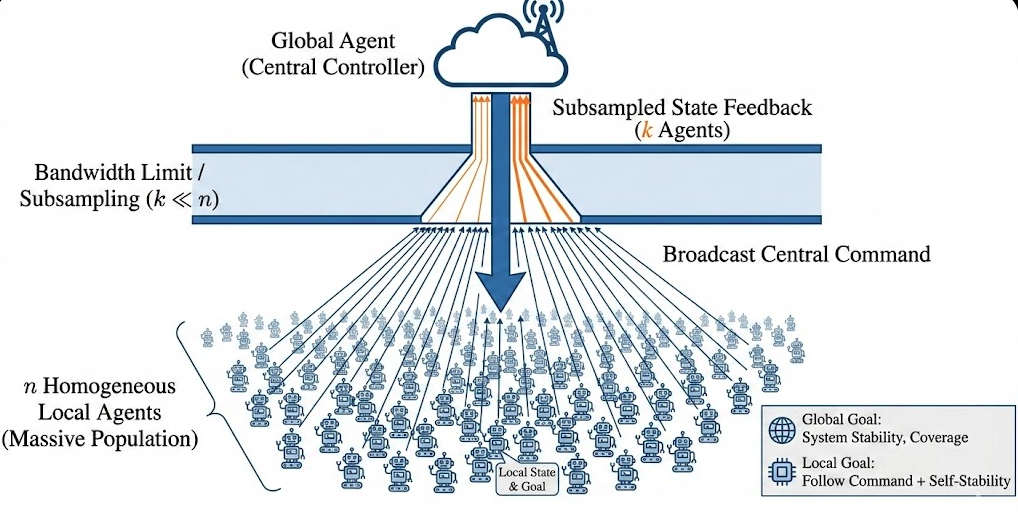
\includegraphics[width=1\linewidth]{sections//Figures/robot2.png}
    \caption{Robot Coordination. This figure illustrates how our communication-constrained framework can be applied for decentralized coordination of large teams of robots. We note that generative AI was used to refine aesthetics of this figure.}
    \label{fig:placeholder}
\end{figure}

\textbf{Mild heterogeneity via finite types.}
While we present the model with homogeneous locals, our framework also supports a finite type space $\mathcal E$. However, as noted in \citep{anand2025meanfield}, using techniques of \citet{10.5555/3586589.3586718}, one can augment each local state as $s_i=(e_i,x_i)\in \mathcal E\times\mathcal X$, allowing rewards and transitions to depend on $e_i$.
All results then scale with the effective local state space size $|\mathcal S_\ell|=|\mathcal E||\mathcal X|$.\looseness=-1
 

\section{Algorithmic Approach: Alternating MARL}\label{sec:approach-algorithms}
 
At a high-level, our approach builds on that of \citet{anand2025meanfield}. However, in order to extend their approach to the communication-constrained setting, we require several technical adaptations to generalize their methods to a Markov game framework. While some of our approach and notation follow the convention of \citet{anand2025meanfield}, the analysis techniques and sub-routines differ substantially. In particular, while Algorithm~\ref{algorithm: g learn} is perhaps similar to \citet{anand2025meanfield}, our work introduces technical novelties in our implementation of Algorithms~\ref{algorithm: l learn} and~\ref{algorithm: alternating marl} as well as their analyses, and the theoretical guarantees of the overall method.

\subsection{Overview of Approach}
 

First, suppose that we fix the local agent's policy $\pi_\ell \in \Pi_\ell$ and optimize the global agent's policy $\pi_g \in \Pi_g$. Then, letting $a_g \sim \pi_g(\cdot|s_g,s_\Delta)$, the transition dynamics are constrained to $s_g' \!\sim\! P_g(\cdot|s_g, a_g)$ and $s_i'\!\sim\!\bar{P}_l^{\pi_\ell}(\cdot|s_g,s_i)$, where 
\begin{equation}\bar{P}_l^{\pi_\ell}(\cdot|s_i, s_g)= P_l(\cdot| s_i, s_g, \pi_\ell( s_i, s_g)).
\label{policy guided transition equation}\end{equation}
Then, optimizing $\pi_g$ under these constrained dynamics corresponds to approximately computing a \emph{best-response} to the pre-fixed policy $\pi_\ell$. Next, we can repeat this procedure, holding $\pi_g$ fixed, and optimizing $\pi_\ell$ in the induced MDP. This alternating procedure forms a sequence of \emph{best-response dynamics}. If the sequence converges, the resultant policy is a Nash equilibrium (by \cref{def: a nash equilibrium}).\looseness=-1


\textbf{Offline Learning:} 
First, in \cref{algorithm: g learn} (\texttt{G-LEARN}), the global agent fixes the local agent's policy $\pi_\ell$. Next, following the techniques of \citet{anand2025meanfield}, the algorithm randomly samples a subset of local agents $\Delta\subseteq [n]$ such that $|\Delta|=k$: it runs value iteration (with $m$ samples) to approximate the $Q$-function \smash{$\hat{Q}_{k,m}^{\text{est}}$} and policy \smash{$\hat{\pi}_{k,m}^{\text{est}}$} for its best-response to $\pi_\ell$ in the surrogate subsystem of $k$ local agents. The surrogate reward of this system, under the fixed local policy $\pi_\ell$, is denoted as \smash{$\bar{r}^{\pi_\ell}_l(s_i, s_g)=r_l(s_i, s_g, \pi_\ell(s_i, s_g))$}, and the stage reward received by the global agent is denoted as \smash{$\bar{r}^{\pi_\ell}_\Delta:\cS\times\cA_g\to\mathbb{R}$}, where
\begin{align}
\bar{r}^{\pi_\ell}_\Delta(s,a_g) = r_g(s_g,a_g)+\frac1{|\Delta|}\sum_{i\in\Delta}\bar{r}^{\pi_\ell}_l( s_i, s_g).
\end{align}
Next, in \cref{theorem: Q-lipschitz of Fsdelta and Fsn}, we prove an analog of Theorem E.3 of \citet{anand2025meanfield}, which shows that $\|\hat{Q}_{k,m}^{\text{est}} - Q^*\|_\infty$ is Lipschitz continuous with respect to the TV-distance between the states of the subsampled agents and the full set of agents, thereby decaying on the order of $\tilde{O}(1/\sqrt{k})$. 


Next, in \cref{algorithm: l learn} (\texttt{L-LEARN}), a representative local agent fixes the global agent's policy $\pi_g$, and learns an approximate best-response in the policy class $\Pi_\ell$ consisting of policies of the form $\smash{\pi_\ell:\cS_g\times\cS_l\to\cA_l}$. However, since the global agent's action depends on a sample of $k$ local agents, the representative local agent's environment is not Markovian in $(s_g, s_i)$. We resolve this by constructing an episodic chained-MDP in \cref{algorithm: k chained induced MDP} and \cref{algorithm: S chained induced MDP} and then applying a standard PAC episodic RL method (UCFH, \cite{dann2015sample}) to extract the local agent's policy.\looseness=-1

Finally, in \cref{algorithm: alternating marl}, \texttt{ALTERNATING-MARL} deploys algorithms \texttt{G-LEARN} and \texttt{L-LEARN}, where algorithm alternately learn a better policy through the induced best-response dynamics process until it converges.

\textbf{Online Execution:} \cref{algorithm: online execution}. To convert the optimality of the global agent's action in the $k$ local-agent subsystem to an approximate optimality guarantee on the full $n$-agent subsystem, we adapt the techniques of \citet{anand2025meanfield} and leverage a randomized policy $\pi_{k,m}^{\text{est}}$ where the global agent samples $\smash{\Delta\in{[n]\choose k}}$ at each time-step to derive an action $\smash{a_g\gets \hat{\pi}_{k,m}^{\text{est}}(s_g, s_\Delta)}$. Synchronously, each local agent $i\in[n]$ evaluates the shared $\pi_\ell$ to get an action $a_i \sim \pi_\ell(\cdot|s_i,s_g)$. We show in \cref{theorem: main result} that the resultant policy is a $\tilde{O}(1/\sqrt{k})$-approximate Nash Equilibrium.   

\subsection{Algorithm Description}

We first introduce the empirical distribution function.

\begin{definition}[Empirical distribution function $F_{s_\Delta}$] \emph{Let $\mu_k(\cS_l) = \{\nu\in\Delta(\cS_l): \nu(x)\in\{0,\frac1k, \frac2k,\dots, 1\}$ be the (discrete simplex) space of $|\cS_l|$-sized vectors. Then, for $\Delta\in {[n]\choose k}$, the empirical distribution function $F_{s_\Delta} \in \mu_k(\cS_l)$ is the proportion of sampled agents at each state, i.e., for $s\in \cS_l, F_{s_\Delta}(s) = \frac1k \sum_{i\in\Delta}\mathbbm{1}\{s_i=s\}$.}\looseness=-1
\end{definition}


\textbf{Offline Learning (I).} We describe \cref{algorithm: g learn} (\texttt{G-LEARN}). Let $m\in\mathbb N$ denote the sample size for the learning algorithm with parameter $k\leq n$. When $|\cS_l|^k \leq |\cS_l|k^{|\cS_l|}$, the algorithm uses traditional value-iteration, and otherwise it uses mean-field value iteration. We formally describe the procedures for each regime below.
\begin{algorithm}[t]
    \caption{\texttt{G-LEARN:} Global-agent $Q$-learning}
    \begin{algorithmic}
        \REQUIRE Global agent transition function $P_g$, local agent policy-guided transition function $\bar{P_l}^{\pi_\ell}$, subsampling parameters $k$ and $m$, and number of Bellman updates $T$.\\
        \STATE Let $\mu_{k}(\cS_l) \coloneqq \{v=\{0, \frac1k, \dots, 1\}^{|\cS_l|}: \sum_i v_i = 1\}$.
        \IF{$|\cS_l|^k \leq |\cS_l|k^{|\cS_l|}$}
        \STATE \textcolor{blue}{\texttt{/$\star$ subsampled standard $Q$-learning}}
        \STATE Set $\hat{Q}_{k,m}^0(s_g, s_\Delta,a_g)\!=\!0, \forall (s_g, s_\Delta, a_g)\!\in\! \mathcal{S}_g\!\times\! \mathcal{S}_l^k\!\times\!  \mathcal{A}_g$.\looseness=-1
        \FOR{$t=0,\dots,T-1$}
\FOR{$s_g,s_\Delta,a_g\in\mathcal{S}_g\times\mathcal{S}_l^k\times\mathcal{A}_g$}
        \STATE $\hat{Q}_{k,m}^{t+1}(s_g,s_\Delta,a_g) = \tilde{T}_{k,m}^{\text{est}}\hat{Q}_{k,m}^t(s_g,s_\Delta,a_g)$
        \ENDFOR
        \ENDFOR
        \ELSE
        \STATE \textcolor{blue}{\texttt{/$\star$ subsampled mean-field $Q$-learning}}
        \STATE \!\!Set $\hat{Q}_{k,m}^0(s_g,F_{ s_\Delta},a_g)=0$
    \FOR{$t=0,\dots,T-1$}
\FOR{$s_g,F_{s_\Delta},a_g\in\mathcal{S}_g\times\mu_k(\cS_l)\times\mathcal{A}_g$}
        \STATE $\hat{Q}_{k,m}^{t+1}(s_g, F_{s_\Delta},a_g) = \hat{T}_{k,m}^{\text{est}}\hat{Q}_{k,m}^t(s_g, F_{s_\Delta},a_g)$
        \ENDFOR
        \ENDFOR
        \ENDIF 
        \STATE Let
 $\hat{\pi}_{k,m}^{T}(\cdot,\cdot)\!=\!\arg\max_{a_g\in\cA_g}\! \hat{Q}_{k,m}^{T}(\cdot,\cdot,a_g)$.
 \STATE Let $V_{\text{new}} = \texttt{APPROX-VALUE}(\hat{\pi}_{k,m}^{T}, \hat{Q}_{k,m}^{T})$.
     \STATE \textbf{return} $\hat{\pi}_{k,m}^{T}$ and $V_{\text{new}}$.
\smallskip
\STATE \textbf{Function} \texttt{APPROX-VALUE}$(\pi_g, \hat{Q}_{k,m})$
\STATE \textbf{if} { $|\cS_l|^k \leq |\cS_l| k^{|\cS_l|}$} 
        \STATE \quad \textbf{for} $s \in \mathcal{S}_g\times \mathcal{S}_l^k$ \textbf{do}
         \STATE \quad\quad  $V_k^{\pi_g}(s) = \sum_{a\in \cA_g} \pi_g(a_g|s))\hat{Q}_{k,m}(s, a_g)$
    \STATE \textbf{else}
   \STATE \quad \textbf{for} $s\in \mathcal{S}_g\times\mu_k(\mathcal{S}_l)$ \textbf{do}
   \STATE \quad\quad $V_k^{\pi_g}(s) = \sum_{a\in \cA_g} \pi_g(a_g|s))\hat{Q}_{k,m}(s, a_g)$
\STATE \textbf{Return $V_k^{\pi_g}$}.
         \label{algorithm: g learn}
    \end{algorithmic}
\end{algorithm}
In the regime where $\smash{|\cS_l|^k\!\leq\!|\cS_l| k^{|\cS_l|}}$, we fix the local agent policy $\pi_\ell$ and learn the best-response $Q$-function for a subsystem with $k$ local agents, denoted by $\hat{Q}_{k,m}^t:\cS_g\!\times\!\cS_l^k\!\times\!\cA_g\!\to\!\mathbb{R}$, which is initialized to $0$. At time $t$, we update 
\begin{align}\hat{Q}_{k,m}^{t+1}(s_g, s_\Delta, a_g) = \tilde{T}_{k,m}\hat{Q}_{k,m}^t(s_g,s_\Delta,a_g),\end{align} where, as in \citet{anand2025meanfield}, $\tilde{T}_{k,m}$ is the empirical adapted Bellman operator, which uses $m$ random samples $s_g^j\sim P_g(\cdot|s_g,a_g)$ and $s_i^j\sim \bar{P_l}^{\pi_\ell}(\cdot|s_i,s_g)$ for each $j\in[m]$.
\begin{align*}\tilde{T}_{k,m}\hat{Q}_{k,m}^t(s_g,s_\Delta,a_g) &= \bar{r}^{\pi_\ell}_\Delta(s,a_g) \\
&+ \frac{\gamma}{m}\sum_{j\in[m]}\max_{a_g'\in\cA_g}\hat{Q}_{k,m}^t(s_g^j, s_\Delta^j,a_g').
\end{align*}
\texttt{G-LEARN} applies value iteration with $\tilde{\cT}$ until $\hat{Q}_{k,m}$ converges to a fixed point satisfying $\smash{\tilde{T}_{k,m}\hat{Q}_{k,m}^{\text{est}} = \hat{Q}_{k,m}^{\text{est}}}$ ($\smash{\tilde{\cT}_{k,m}}$ is $\gamma$-contractive), converging to a deterministic policy $\hat{\pi}_{k,m}^{\text{est}}$,
\begin{equation}\hat{\pi}_{k,m}^{\text{est}}(s_g,s_\Delta) = \arg\max_{a_g\in\mathcal{A}_g} \hat{Q}_{k,m}^{\text{est}}(s_g, s_\Delta, a_g).\end{equation}
When $\smash{|\cS_l|^k\!>\!|\cS_l|k^{|\cS_l|}}$, the mean-field MARL transformation is helpful in reducing complexity, and hence we learn the mean-field best-response $Q$-function, $\hat{Q}_{k,m}^t:\cS_g\!\times\!\mu_{k}(\cS_l)\!\times\!\cA_g\!\to\!\mathbb{R}$. Initializing at $0$, we iteratively perform the update in the empirical distribution parameterization:
\begin{align}\hat{Q}_{k,m}^{t+1}(s_g, F_{s_\Delta}, a_g) = \hat{T}_{k,m}\hat{Q}_{k,m}^t(s_g, F_{s_\Delta}, a_g),\end{align}
where $\hat{T}_{k,m}$ is the empirical adapted mean-field Bellman operator in the mean-field parameterization: 
\begin{align*}
    \hat{\cT}_{k,m}\hat{Q}_{k,m}^t & (s_g, F_{s_\Delta},a_g) = \bar{r}^{\pi_\ell}_\Delta(s,a_g) \\
    &\quad\quad + \frac{\gamma}{m}\sum_{j\in[m]}\max_{a_g'\in\cA_g}\hat{Q}_{k,m}^t(s_g^j, F_{s_\Delta^j},a_g'),
\end{align*}
 which admits the same fixed point $\hat{Q}_{k,m}^{\text{est}}$ and policy $\hat{\pi}_{k,m}^{\text{est}}$.
 

\textbf{Offline Learning (II).} For \cref{algorithm: l learn} (\texttt{L-LEARN}), we fix the global agent's policy $\pi_g$. Then, a representative local agent faces an induced MDP with state space
$\mathcal{S}_l \times \mathcal{S}_g$, action space $\mathcal{A}_l$, transition kernel inherited from the game,
and reward scaled by $1/n$.  Since the global agent's action depends on a sample of $k$ local agents, the representative local agent's environment is not Markovian in $(s_g, s_i)$. We resolve this by constructing an episodic chained-MDP in Algorithms \ref{algorithm: k chained induced MDP} and \ref{algorithm: S chained induced MDP}. The difficulty here is that the global agent's policy $\pi_g$ requires a $k$-tuple of local states whereas a single local agent only sees $s_{g}$ and $s_{i}$. Our reduction resolves this by explicitly maintaining a $k$-tuple of local states and serializing the $k$ local decisions within each macro step such that where each agent uses the same policy which maps from $\mathcal{S}_l\times\mathcal{S}_g\to\mathcal{A}_l$. \looseness=-1


\begin{algorithm}[t]
\caption{\texttt{L-LEARN}: Local-agent $Q$-learning}
    \begin{algorithmic}
        \REQUIRE Transition kernels $P_l, P_g$, fixed global-agent policy $\pi_g$, parameters $k$ and $\gamma$,  and failure probability. $\delta_\ell$.
        \STATE Set $H\coloneqq \frac{1}{1-\gamma}\log \frac{\|r\|_\infty\sqrt{k}}{1-\gamma}$ as the effective horizon.
        \STATE \textcolor{blue}{\texttt{/$\star$ Form a proxy episodic MDP $\smash{\widetilde{M}_k(\pi_g)}$}}
        \STATE \textbf{if} { $|\cS_l|^k \leq |\cS_l| k^{|\cS_l|}$} 
        \STATE \quad \textcolor{blue}{\texttt{/$\star$ standard parameterization}}
        \STATE \quad Use \cref{algorithm: k chained induced MDP}  to construct the $k$-chained MDP $\widetilde M_k$ 
        \STATE \quad with horizon $\widetilde H = H\cdot k$ 
        \STATE \textbf{else} 
        \STATE \quad \textcolor{blue}{\texttt{/$\star$ mean-field parameterization}}
        \STATE \quad Use \cref{algorithm: S chained induced MDP} to construct the $|\mathcal S_l|$-chained mean-
        \STATE \quad field MDP $\widetilde M_{k}$ with horizon $\widetilde H = H\cdot(|\mathcal S_l|+1)$.
        \smallskip
        \STATE Run an episodic PAC RL solver (e.g., UCFH) on $\widetilde{{M}}_k(\pi_g)$ with parameters $\epsilon_\ell=\frac{1}{\sqrt{k}}, \delta_\ell$ to obtain induced policy $\pi_\ell$.
        \STATE \textbf{Return} policy $\pi_\ell$ and value function estimate $\widehat{V}^{\pi_\ell, \pi_g}$.
    \end{algorithmic}
    \label{algorithm: l learn}
\end{algorithm}

Specifically, \cref{algorithm: k chained induced MDP} replaces each macro time step $t$ by a chain of $k$ micro steps $\smash{\tau = tk, tk+1, \dots, tk+(k-1)}$, indexed by a stage pointer $\smash{j\in\{1,\dots,k\}}$. The state of the unfolded system at micro step $\tau$ is given by $\smash{(j, s_g, \bar{s}_g, s_{1:k})}$, where $s_{1:k}$ are the local ``replica'' states, $s_g$ is the current global state, and $\bar{s}_g$ is a pending next global state. At the first micro node of each chain (where the stage $j=1$ and $\bar{s}_g = \perp$), we evaluate the global agent's policy using the entire replica tuple and compute $\smash{a_g\sim \pi_g(\cdot|s_g, s_{1:k})}$, and sample a pending global next state $\smash{\bar{s}_g\sim P_g(\cdot|s_g, a_g)}$. This pending global transition is computed before updating any local replica, making it consistent with the original macro-step semantics. Along the chain of micro nodes, only one local replica is ``active'' at any time. At stage $j$, the learner selects the action for replica $\smash{j, a_\ell\in\mathcal{A}_l}$. The environment updates that replica via $\smash{s_j' \sim P_l(\cdot|s_j, s_g, a_\ell)}$, leaving the other local replica states unchanged, and increments $j$. At stage $j=k$, it commits the cached global transition, setting $s_g\!\gets\! \bar{s}_g$ and resetting $\bar{S}_g \gets \perp$, completing one macro step.

Similarly, in the mean-field parameterization in \cref{algorithm: S chained induced MDP}, we maintain an empirical distribution on the number of agents at each state: if $h(u)$ agents occupy state $u\in\mathcal{S}_l$, we apply the local action $a_\ell$ for state $u$ to move the mass $h(u)$ to next states via the multinomial induced by $P_l(\cdot|u,s_g,a_\ell)$, accumulating these counts in a new histogram $\bar{F}_\Delta$.  Finally, we run UCFH \cite{dann2015sample} which is an episodic PAC RL solver on the constructed MDP $\widetilde{\cM}_k(\pi_g)$ to obtain an $\epsilon_\ell$ best-response induced policy $\pi_\ell$. 

\textbf{Offline Learning (III).} \texttt{ALTERNATING-MARL} in \cref{algorithm: alternating marl} orchestrates alternating best-responses of \texttt{G-LEARN} and \texttt{L-LEARN} for $N_{\text{steps}}$-many iterations: each algorithm proposes its best-response policy, and \cref{algorithm: alternating marl} accepts the policy if it estimates that it has improved the joint value function, up to a tolerance radius of $\smash{\tilde{O}(1/\sqrt{k})}$. To ensure that the potential drifts upward on every accepted update, we introduce function \texttt{UPDATE} in \cref{algorithm: alternating marl}, which rejects worse joint policies and terminates the algorithm earlier if a learned best-response policy is within the tolerance radius.\looseness=-1
 

\begin{algorithm}[t]
\begin{algorithmic}
\caption{\texttt{ALTERNATING-MARL}} 
\REQUIRE Transition functions $P_g$ and $P_\ell$, initial uniform policies $(\pi_g^0,\pi_\ell^0)$, steps $N_{\text{steps}}$,   failure probability $\delta$, algorithms \texttt{G-LEARN} and \texttt{L-LEARN}, and sampling parameters $k$ and $m$.
\smallskip
\STATE Set $\delta_{\text{learn}} = \frac{\delta}{4N_{\text{steps}}}$ and $T=\frac{2}{1-\gamma}\log\frac{\tilde{r}\sqrt{k}}{1-\gamma}$.\\
\STATE Set $\hat{V}_{\text{old}} = 0$.\\
\smallskip
\FOR{$t=1,\dots,N_{\text{steps}}$}
\smallskip
\STATE \textcolor{blue}{\texttt{/$\star$ Propose a policy update to $\pi_g$}}\smallskip
\STATE Form  $\bar{P}_l\coloneqq \smash{\bar{P}_l^{\pi_\ell^{t-1}}}$ using Equation \ref{policy guided transition equation}.
\STATE $ \tilde\pi_g, \hat{V}_{\text{new}} \leftarrow \texttt{G-LEARN}
(P_g,\bar{P}_\ell,k,m,T)$ 
\STATE $\smash{\pi_g^t, \textsc{Nash}, \hat{V}_{\text{old}}} \gets 
\texttt{UPDATE}(\tilde{\pi}_g, \pi_g^{t-1}, \hat{V}_{\text{new}}, \hat{V}_{\text{old}})$
\STATE \textbf{if} \textsc{Nash} = \textsc{True} \textbf{then}
\STATE \quad \textbf{return} $(\pi_g^t, \pi_\ell^{t-1})$
\smallskip
\STATE \textcolor{blue}{\texttt{/$\star$ Propose a policy update to $\pi_\ell$}}
  \STATE $\tilde\pi_\ell, \hat{V}_{\text{new}} \leftarrow \texttt{L-LEARN}(P_g,P_\ell,\pi_g^t,k, \delta_{\text{learn}})$.
  \STATE $\pi_\ell^t, \textsc{Nash}, \hat{V}_{\text{old}} \gets \texttt{UPDATE}(\tilde{\pi}_\ell, \pi_\ell^{t-1},  \hat{V}_{\text{new}}, \hat{V}_{\text{old}})$
  \STATE \textbf{if} \textsc{Nash} = \textsc{True} \textbf{ then }
  \STATE \quad\quad \textbf{return} $(\pi^t_g, \pi^t_\ell)$
  \ENDFOR
\STATE \textbf{return} $(\pi_g^{N_{\text{steps}}},\pi_\ell^{N_{\text{steps}}})$
\smallskip
\STATE \textbf{Function} \texttt{UPDATE}$(\pi_{\text{new}}, \pi_{\text{old}}, \hat{V}_{\text{new}}, \hat{V}_{\text{old}})$
\STATE \quad Let ${\eta = \frac{2\tilde{r}}{(1-\gamma)^2}\left(\sqrt{\frac{1}{2k} \ln(2|\mathcal{S}_l||\mathcal{A}_g|\sqrt{k})} + \frac{5}{\sqrt{k}}\right)}$.
\STATE \quad \textbf{if} {$\hat{V}_{\text{new}} > \hat{V}_{\text{old}} + 2\eta$} on all subsampled states \textbf{then}
\STATE \quad\quad \textbf{return} $(\pi_{\text{new}}, \textsc{False}, \hat{V}_{\text{new}})$  \textcolor{blue}{\texttt{/$\star$ accept}}
\STATE \quad \textbf{else if} {$\hat{V}_{\text{new}} < \hat{V}_{\text{old}} - 2\eta$} on some state \textbf{ then }
\STATE \quad\quad \textbf{return} $(\pi_{\text{old}}, \textsc{False}, \hat{V}_\text{old})$\quad  \textcolor{blue}{\texttt{/$\star$ reject}}
\STATE \quad \textbf{else  }  
\STATE\quad\quad  \textbf{return} $(\pi_{\text{old}}, \textsc{True}, \hat{V}_\text{old})$  \textcolor{blue}{\texttt{/$\star$ terminate}}
\label{algorithm: alternating marl}
\end{algorithmic}
\end{algorithm} 
    
\textbf{Online Execution:} \cref{algorithm: online execution}  (Online execution). To convert the optimality of the global agent's action in the $k$ local-agent subsystem to an approximate optimality guarantee on the full $n$-agent subsystem, we propose a randomized policy $\smash{\pi_{k,m}^{\text{est}}}$ where the global agent samples $\smash{\Delta\in{[n]\choose k}}$ at each time-step to derive an action $\smash{a_g\gets \hat{\pi}_{k,m}^{\text{est}}(s_g, s_\Delta)}$. Synchronously, each local agent $\smash{i\in[n]}$ evaluates the shared $\smash{\pi_\ell}$ to get an action ${a_i \sim \pi_\ell(\cdot|s_i,s_g)}$. \cref{theorem: main result} shows that the resultant policy is a $\tilde{O}(1/\sqrt{k})$-approximate NE.\looseness=-1

\begin{algorithm}
    \caption{Online execution stage}
    \begin{algorithmic}
        \REQUIRE Policies $\pi_g$ and $\pi_\ell$, and states $s_g(0), s_{[n]}(0)\!\sim\!s_0$.
        \STATE Let $R \gets 0$
        \FOR{$t=0,\dots,T-1$}
        \STATE Sample $\Delta\subseteq {[n]\choose k}$ uniformly at random
        \STATE Let $a_g(t) \sim \hat{\pi}_{g,k}(\cdot|s_g(t), s_\Delta(t))$
        \STATE For all $i\in[n]$, let $a_i(t) \sim \pi_\ell(\cdot|s_i(t),s_g(t))$
        \STATE Collect a reward $r_t\!=\! r_g(s_g,a_g)\!+\!\frac1n \sum_{i=1}^n\! r_l(s_i,s_g,a_i)$
        \STATE Let $R \gets R + \gamma^t r_t$
        \STATE The agents transition to their next states
        \ENDFOR
        \label{algorithm: online execution}
    \end{algorithmic}
\end{algorithm}

% \newpage

\section{Theoretical Guarantees and Analysis}

 We begin by giving theoretical guarantees for \texttt{G-LEARN.}

\begin{definition}[Bellman noise] \emph{We first introduce the notion of Bellman noise. Note that $\hat{\cT}_{k,m}$ is an unbiased estimator of the adapted Bellman operator $\hat{\cT}_k$,
\begin{align*}\hat{\mathcal T}_k \hat{Q}_k(s_g, s_\Delta, a_g)
&\coloneqq
\bar{r}^{\pi_\ell}_\Delta(s,a)
\\
&+\gamma\mathbb E_{(s_g',s_\Delta')\sim \mathcal P_k} \max_{a_g'\in\cA_g} \hat{Q}_k(s_g',s_\Delta',a_g')],
\end{align*}
where $\mathcal P_k\!\coloneqq\!P_g\!\otimes\!(\bar{P}^{\pi_\ell}_l)^{\otimes k}$. Here, $\hat Q_k$ is initialized to $0$ and at time $t$ we update $\hat{Q}_k^{t+1}\!=\!\hat{\cT}_k \hat{Q}_k^t$. Similarly, $\hat{\cT}_k$ is a $\gamma$-contraction and admits a fixed point $\hat{Q}_k^*$. By the law of large numbers, as $m\!\to\!\infty$, $\hat{\cT}_{k,m}\!\to\!\hat{\cT}_k$ and $\hat{Q}^*_{k,m}\!\to\!\hat{Q}^*_k$. For finite $m$, $\epsilon_{k,m}\coloneqq \|\hat{Q}_{k,m}^{\text{est}} - \hat{Q}_k^*\|_\infty$ is the Bellman noise.}\looseness=-1
\end{definition}

Then, \cref{theorem: g-learn preliminary} provides a high-probability bound on the approximate best-response of the learned policy.

\begin{theorem}\label{theorem: g-learn preliminary} For all $s\in\cS_g\times\cS_l^n$, if $T\geq\frac{2}{1-\gamma}\log\frac{\tilde{r}\sqrt{k}}{(1-\gamma)}$ in \emph{\texttt{G-LEARN}}, then
\begin{align*}V^{\pi^*}(s)\!&-\! V^{{{\pi}}^\est_{k,m}}(s) \leq \frac{2\epsilon_{k,m}}{1-\gamma} + \frac{2\tilde{r}}{k(1-\gamma)^2}\!\\
&\quad\quad\quad\quad\quad\quad\quad+\! \frac{2\tilde{r}}{(1-\gamma)^2}\sqrt{\frac{1}{2k} \ln 2k |\mathcal{S}_l||\cA_g|}.
\end{align*}
\end{theorem}
We defer the proof of \cref{theorem: g-learn preliminary} to \cref{sec: optimality of global agent policy}, and generalize the result to stochastic rewards in \cref{stochastic generalization}. To bound $\epsilon_{k,m}$, we specify the number of samples $m$ required to control the Bellman noise in \cref{lemma: controlling bellman noise}.

\begin{lemma}
    [Controlling the Bellman noise]\label{lemma: controlling bellman noise} For $k\in[n]$, let \smash{$m_1 \geq  \tilde{O}(\frac{k^2 \gamma^2 \tilde{r}^2 |\cS_l|}{(1-\gamma)^4})$} be the number of samples in the mean-field parameterization and \smash{$m_2 \geq \tilde{O}(\frac{\tilde{r} k^2 \gamma^2}{(1-\gamma)^4})$} be the number of samples in the standard parameterization. Then, we have that with probability at least $1-\frac{1}{100e^k}$,  $\epsilon_{k,m}\leq \frac{2}{\sqrt{k}}$.\looseness=-1
\end{lemma}
We defer the proof of \cref{lemma: controlling bellman noise} to Appendix \ref{lemma: epsilon_km_is_k}. Then, combining \cref{theorem: g-learn preliminary} and \cref{lemma: controlling bellman noise},  we have

\begin{theorem}
    [Global agent subsampling result] \label{theorem: g-learn}
    Let $m^*$ be chosen as in \cref{lemma: controlling bellman noise}, and set $\pi_{k}^{\text{est}} \coloneqq \pi^{\text{est}}_{k,m^*}$. Then, for all $s\in\mathcal{S}$, we have that with probability at least $1-\frac{1}{100e^k}$: \label{theorem: application of PDL}
\begin{align*}V^{\pi^*}(s) &- V^{{{\pi}}^\text{est}_{k}}(s) \\ &\leq {O}\left(\frac{\tilde{r}}{\sqrt{k}(1-\gamma)^2}\sqrt{ \ln(2|\mathcal{S}_l||\mathcal{A}_g|\sqrt{k})} + \frac{2}{\sqrt{k}}\right).
\end{align*}
\end{theorem}

The sample complexity of \texttt{G-LEARN} under standard parameterizations is $\tilde{O}(\frac{k^4\gamma^2 \tilde{r}^2 |\cS_g| |\cS_l|^k |\cA_g|}{(1-\gamma)^5})$, and in mean-field parameterization it is $\tilde{O}(\frac{k^{3+|\cS_l|}\gamma^2\|r_l\|^2_\infty |\cS_g| |\cS_l|^2 |\cA_g|}{(1-\gamma)^5})$.

\begin{remark} We also extend the formulation of \texttt{G-LEARN} to off-policy $Q$-learning \cite{chen2021lyapunov,chen2022sample}, which replaces the generative oracle assumption with a stochastic approximation scheme that learns an approximately optimal policy using historical data. \cref{Appendix/off-policy} provides theoretical guarantees with a similar decaying optimality gap as in \cref{theorem: performance_difference_lemma_applied}. \end{remark}


\subsection{Convergence Guarantees on \texttt{L-LEARN}}

\begin{theorem}[Local agent best-response optimality and sample-complexity guarantees] \label{theorem: l-learn}With probability at least $1-\delta$, the local-agent's learned policy is an $\epsilon$ best-response to the global agent's fixed policy $\pi_g$ with sample complexity
\[\tilde{O}\!\left(\!\min\!\left\{\!\frac{|\cS_l|^5|\cS_g|^2 k^{2|\cS_l|}|\cA_l|}{\epsilon^2(1-\gamma)^2} \!\ln\!\frac1\delta, \frac{k^5  |\cS_g|^2 |\cS_l|^k |\cA_l|}{\epsilon^2(1-\gamma)^3}\!\ln\!\frac1\delta\!\right\}\!\right).\]   
\end{theorem} 

We defer the proof of \cref{theorem: l-learn} to Appendix \ref{appendix theorem: local agent br optimality}, and use these results to analyze \texttt{ALTERNATING-MARL}.

 \subsection{Convergence Guarantees on {\texttt{ALTERNATING-MARL}}}


The dynamics of the meta-algorithm induces a Markov game (also called a \emph{stochastic game}), where the play proceeds by steps from position to position, according to transition probabilities controlled jointly by the agents.

\begin{definition}[Markov Potential games] \emph{Denote the global agent by index $0$, and let the policy of agent $i\in\{0,\dots,n\}$ be denoted by $\pi_i$, and the joint policies of all the other agents be given by $\pi_{-i}$. Then, a stochastic game $\mathcal{M}$ is a Markov Potential Game if there exists a potential function $\Phi:\mathcal{S}\times\mathcal{A}\to\mathbb{R}$ such that for any agent $i\in\{0,\dots,n\}$ and any pair of policies $(\pi_i, \pi_{-i}), (\pi_i', \pi_{-i})$ at any starting state $s_0$, we have that\looseness=-1
\begin{align*}&\mathbb{E}_{\pi'_i,\pi_{-i}}\bigg[\sum_{t=0}^\infty \gamma^t r_i(s_t,a_t) | s_0\bigg]\!-\! \E_{\pi}\bigg[\sum_{t=0}^\infty \gamma^t r_i(s_t,a_t) | s_0\bigg] \\
&\!=\! \mathbb{E}_{\pi'_i,\pi_{-i}}\bigg[\sum_{t=0}^\infty \gamma^t \Phi(s_t,a_t)| s_0\bigg]\!-\! \E_{\pi}\bigg[\sum_{t=0}^\infty \gamma^t \Phi(s_t,a_t)|s_0\bigg],
\end{align*}
i.e., when agent $i$ switches from policy $\pi_i$ to policy $\pi'_{i}$, $\Delta\Phi$ equals the change in the utility of that player's policy.}
\end{definition}

We show that the Markov game in our setting is a {Markov Potential game} in \cref{lemma: M is a Markov potential game} and exploit a theorem of \citet{doi:10.1073/pnas.39.10.1095} that best-response dynamics converge to pure Nash Equilibria in Markov potential games. However, unlike the continuous time dynamics which converges rapidly \cite{doi:10.1137/17M1139461}, the worst-case bound in the discrete-time dynamics can converge exponentially slowly in the number of players \cite{DurandGaujal:2016:ACBRA}. However, under homogeneity, the $(n+1)$-player game restricted to the policy class $\Pi_g$ and $\Pi_\ell$ is equivalent to a $2$-player game between the global agent and a representative local agent, yielding a dimension-reduced dynamic that converges rapidly towards a Nash Equilibrium in \cref{theorem: main result}.\looseness=-1

\begin{theorem}[The sample complexity of learning a $2\eta$-approximate Nash Equilibrium] \label{theorem: main result}
Fix $\delta\in(0,1)$, and let $\eta=\max\{\epsilon_g, \epsilon_l\}$ be the maximum error incurred by Algorithms \emph{\texttt{G-LEARN}} and \emph{\texttt{L-LEARN}}. Then, we have \begin{align*}\eta\! &=\!\frac{2\tilde{r}}{(1\!-\!\gamma)^2}\left(\sqrt{\frac{1}{2k} \ln(2|\mathcal{S}_l||\mathcal{A}_g|\sqrt{k})}\!+\!\frac{5}{\sqrt{k}}\right)\!\leq\!\tilde{O}\left(\frac1{\sqrt{k}}\right).
\end{align*}
Setting $N_{\text{steps}} = 2|\cS_g|^2 |\cA_g| |\cA_l| \cdot \min\{|\cS_l|^2 k^{|\cS_g|},  |\cS_l|^{k+1}\}$, \emph{\texttt{ALTERNATING-MARL}} learns a  $2\eta$-approximate NE with probability at least $1-\delta$,  and sample complexity.
\begin{align*}
\tilde{O}\bigg(\!&\min\bigg\{\frac{|\mathcal{S}_g|^4|\mathcal{A}_g|^2 |\cA_l|^2 |\mathcal{S}_l|^8 k^{3 + 3|\mathcal{S}_l| }\tilde{r}}{(1-\gamma)^5}\log \frac1\delta, \\ &\quad\quad\quad\quad\quad\quad \frac{|\cS_g|^4 |\cS_l|^{2k+1} |\cA_g|^2 |\cA_l|^2 k^7 \tilde{r}^2}{(1-\gamma)^5} \log \frac{1}{\delta} \bigg\}\bigg),
\end{align*}
\end{theorem}

\begin{remark}[Tradeoff in $k$ and the Rewards of Subsampling]\label{remark: tradeoff in k} In the mean-field parameterization, our bound in \cref{theorem: main result} dismantles the exponential dependence on the size of the action space of the local agents. In the standard parameterization, our bound removes the dependence on the size of the joint action space of the local agents that had existed in prior works \cite{yang2020meanfieldmultiagentreinforcement,li2021permutationinvariantpolicyoptimization, gu2021meanfieldcontrolsqlearningcooperative,gu2022meanfieldmultiagentreinforcementlearning,anand2025meanfield}. By \cref{theorem: main result}, we observe that as $k\to n$, the approximate Nash Equilibrium approaches a Nash Equilibrium, revealing a fundamental trade-off in the choice of $k$: increasing $k$ improves the performance of the policy, but increases the size of the $\hat{Q}_k$-function.  Importantly, our sample complexity breaks the exponential dependence on the number of agents on the action space, while attaining only a logarithmic dependence on the agents in terms of the state space: if we set $k=O(\log n)$, we get a sample complexity of $\tilde{O}(|\cS_g|^4 |\cA_g|^2 |\cA_l|^2 \cdot \min\{|\cS_l|^8 (\log n)^{|\cS_l|}, |\cS_l|^{\log n}\})$ with decaying optimality gap on the order of $1/\sqrt{\log n}$.\looseness=-1
\end{remark}


\begin{remark} The polynomial dependence on the effective horizon $\frac{1}{1-\gamma}$ in our work is likely loose. This is because we did not attempt to leverage more sophisticated variance-reduction techniques \citep{sidford2018near,Sidford2018VarianceRV, wainwright2019variance, jin2024truncated}. While we believe our techniques can likely be combined with variance reduction to improve this dependence on $\frac{1}{1-\gamma}$; we omit this from this paper because our focus is on the reducing dependence on $n$ rather than the discount factor.\looseness=-1
\end{remark}

\section{Conclusion and Future Work}
We introduce a mean-field framework for communication-constrained multi-agent reinforcement learning by formulating this problem as best-response dynamics under a Markov game. We propose \texttt{ALTERNATING-MARL}, which learns each agent’s best response to the mean effect of the local agents policies from $k$ samples of the local agents. This enables an exponential reduction in the sample complexity of approximating a solution to the MDP. We prove that the resultant policy is a $\smash{\tilde{O}(\frac{1}{\sqrt{k}})}$-approximate Nash equilibrium. We extend our result to the off-policy learning setting with stochastic rewards, and validate our theory with numerical simulations in communication-constrained control settings.

\textbf{Limitations and future work.} 
We assume that the global and local agents cooperate to optimize a structured reward under a specific dynamic model which was studied in \citet{anand2025meanfield}. A natural direction for future is to explore the extent to which our algorithms and analysis can be extended to weaker assumptions on the dynamics model or the reward structure. Second, our work is only able to incorporate mild heterogeneity among cooperative agents. It would be interesting to explore the extent to which we can capture a greater degree of heterogeneity \cite{Hu_Wei_Yan_Zhang_2023,cui2022learning,anand2026graphonmeanfieldsubsamplingcooperative,wang2026unsuperviseddecompositionrecombinationdiscriminatordriven}. Finally, it would be exciting to generalize this work to the setting with infinite/continuous state spaces with general function approximation. This would require more technical algorithms using least-squares value iteration \cite{xu2023tale, ayoub2020model} or linearity assumptions on the underlying MDP \cite{golowich2024linear,  golowich2024the}.\looseness=-1
 
% \newpage

\section*{Impact Statement}
This paper contributes to the theoretical foundations of MARL, with the goal of developing mean-field tools that can apply to the control of networked systems. The work can potentially lead to algorithms to adaptively control of cyber-physical systems. Furthermore, any applications of the proposed algorithm in its current form should be considered cautiously since the analysis here focuses on efficiency and stationarity, but does not consider issues of fairness in the vector-reward framework \cite{pmlr-v19-abernethy11b}.


